\documentclass{article}   	% use "amsart" instead of "article" for AMSLaTeX format
\usepackage{geometry}                		% See geometry.pdf to learn the layout options. There are lots.
\geometry{letterpaper}                   		% ... or a4paper or a5paper or ... 
\usepackage{graphicx}				% Use pdf, png, jpg, or eps§ with pdflatex; use eps in DVI mode
\usepackage{amsmath}
\usepackage{amssymb}
\usepackage{natbib}
\usepackage{lineno}
\usepackage{color}
\usepackage{hyperref}
\linenumbers


\title{DESI Observations of Type Ia Supernovae Discovered by Imaging Surveys}


\begin{document}
\maketitle

\section{Host Redshifts of ZTF Discoveries with Good Light Curves}
ZTF will discover SNe~Ia that ultimately get ``good'' light curve measurements.  ZTF is expected to have discovery completeness to $z=0.15$.
For an imagined survey that overlaps ZTF and DESI fields, Nordin has estimated the
numbers of SN~Ia discoveries, the numbers of those with good light curves, and the numbers with redshifts from the SED~Machine.
The estimates are shown in Figure~\ref{ZTFnum:fig}.  (I presume some SNe with redshifts don't have good light curves.) 
The DESI footprint
is 14,000 square degrees.  Assuming that the 961 supernovae with good light curves are distributed uniformly, there will be 0.069
of these per square degree, or 0.5 per instrumented 7.5 square degree  DESI footprint.


\begin{figure}[h]
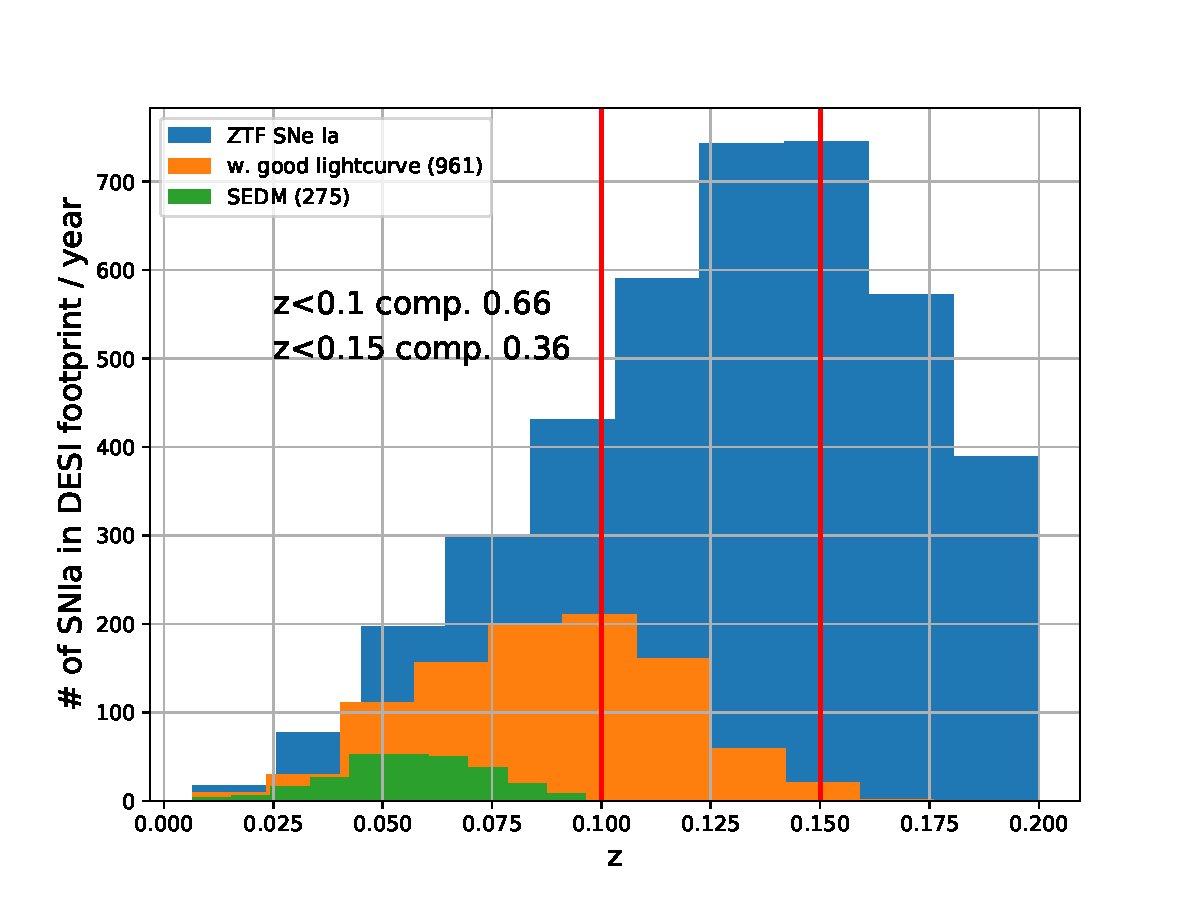
\includegraphics[width=8cm]{zdist_12m_185_195.pdf}
\centering
\caption{Numbers of ZTF SN~Ia discoveries, the numbers of those with good light curves, and the numbers with redshifts from the SED~Machine.
\label{ZTFnum:fig}}
\end{figure}

Redshifts of the host galaxies will be obtained using the SED~Machine, serendipitously as a DESI Bright Galaxy Survey (or other) target.
More redshifts could be obtained using spare fibers available during the DESI survey.

A rough estimate (calculated
using mock.py)
of the fraction of supernovae in a DESI BGS field 
that occur in a host galaxy with a successful DESI redshift is shown in Figure~\ref{19.5:fig}.
At redshift $z=0.15$, where ZTF is complete and the upper-redshift limit for objects with good light curves, half of ZTF supernovae will have a DESI redshift.
At redshift $z=0.1$, where the distribution of supernovae with good light curves peaks, 70\% of ZTF supernovae will have a DESI redshift.
That fraction increases to near-completeness as redshift decreases to zero.
The vast majority of missing redshifts are
because the host galaxy is too faint to be targeted in the BGS survey.
The remaining effects are
a 97 (92)\% efficiency for fiber allocation and a 92 (77)\% efficiency of extracting a redshift from the data for Tier 1(2) targets. 

\begin{figure}[h]
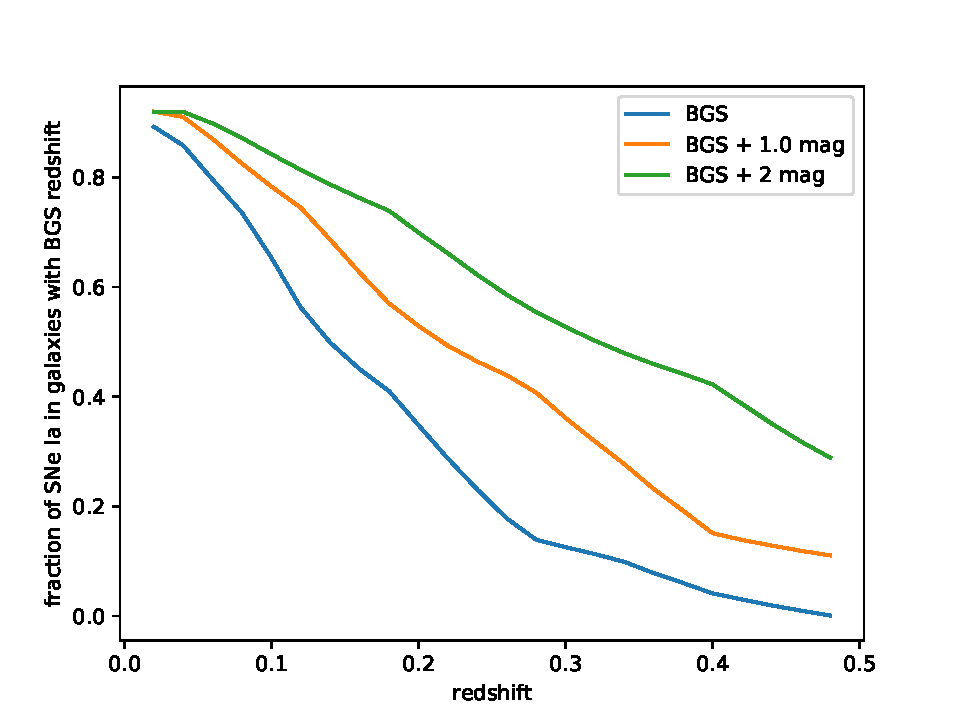
\includegraphics[width=8cm]{bg_frac.pdf}
\centering
\caption{Fraction of supernovae in a DESI BGS field 
that occur in a host galaxy with a successful DESI redshift.  Also shown are the fraction of supernovae that would occur in a host galaxy
with a successful DESI redshift (assuming 100\% fiber-allocation efficiency) shifting the efficiencies 1 and 2 mag deeper than the nominal BGS exposure.
\label{19.5:fig}}
\end{figure}

A candidate program to obtain redshifts of hosts not obtained by the BGS is to target host galaxies down to a fainter magnitude limit.
Figure~\ref{19.5:fig} shows the fractions of supernovae that would occur in a host galaxy
with a successful DESI redshift (now assuming 100\% fiber-allocation efficiency) shifting the efficiencies 1 and 2 mag deeper than the nominal BGS exposure.
(I believe that the standard DESI survey is 2-mag deeper than the BGS.)
At redshift $z=0.15$,  $\sim 80$\% of ZTF supernovae could get a DESI redshift going 2-magnitudes deeper than BGS.
At redshift $z=0.1$, 90\% of ZTF supernovae will have a DESI redshift.


Summary: Over the course of its survey, ZTF will discover $\sim 960$ SNe~Ia with good light curves.  With a matched field of view,
the DESI BGS survey will ``automatically'' obtain redshifts of a fraction of the brightest galaxies in the field, so that a significant majority
of supernovae with good light curves will have a redshift.   By targeting supernova host galaxies down to a fainter limiting magnitude,
DESI could increase the number of host-galaxy redshifts be a factor $\sim 2$ at the extreme redshift of $z=0.15$.  The number of targets would be
$\ll 0.25$ per DESI footprint.

\section{Triggered Followup of Active Type Ia Supernovae}
DESI can classify active SNe~Ia in its spectra, say of
a transient discovered by an imaging survey and  observed as a DESI secondary target.
For the nominal target depths of its surveys, the DESI classification efficiency curve approximates 
a unit step function with perfect classification success/failure when brighter/fainter than some $r$ limiting magnitude.  (Graur and Moustakas are recalculating these.)

To see how many objects DESI could classify in a single pointing, 
it is of interest to know how many SNe~Ia are brighter than some magnitude at any given moment.
Shown in Figure~\ref{cum:fig} are cumulative number densities of SNe~Ia that are instantaneously brighter than a limiting magnitude as a function of redshift.
Several limiting magnitudes are considered. 
As the limiting magnitude increases, the number density asymptotes at higher values and redshifts.  For the shallow $r_{lim}=19.5$~mag limit the density plateaus at $z \sim 0.1$ with $2\times 10^{-3}$ objects per square degree or 0.015 per DESI footprint.   For the $r_{lim}=21.5$~mag limit the plateau occurs at $z \sim 0.3$ with $3.4\times 10^{-2}$ objects per square degree or 0.26 per DESI footprint.  Correspondingly, roughly one in 67 (4) DESI pointings will have a measurable SN~Ia in its footprint.
The majority of transients at these magnitudes and high Galactic latitude will be SNe~Ia, so considering all transients would have only a small increase total rates.

\begin{figure}[h]
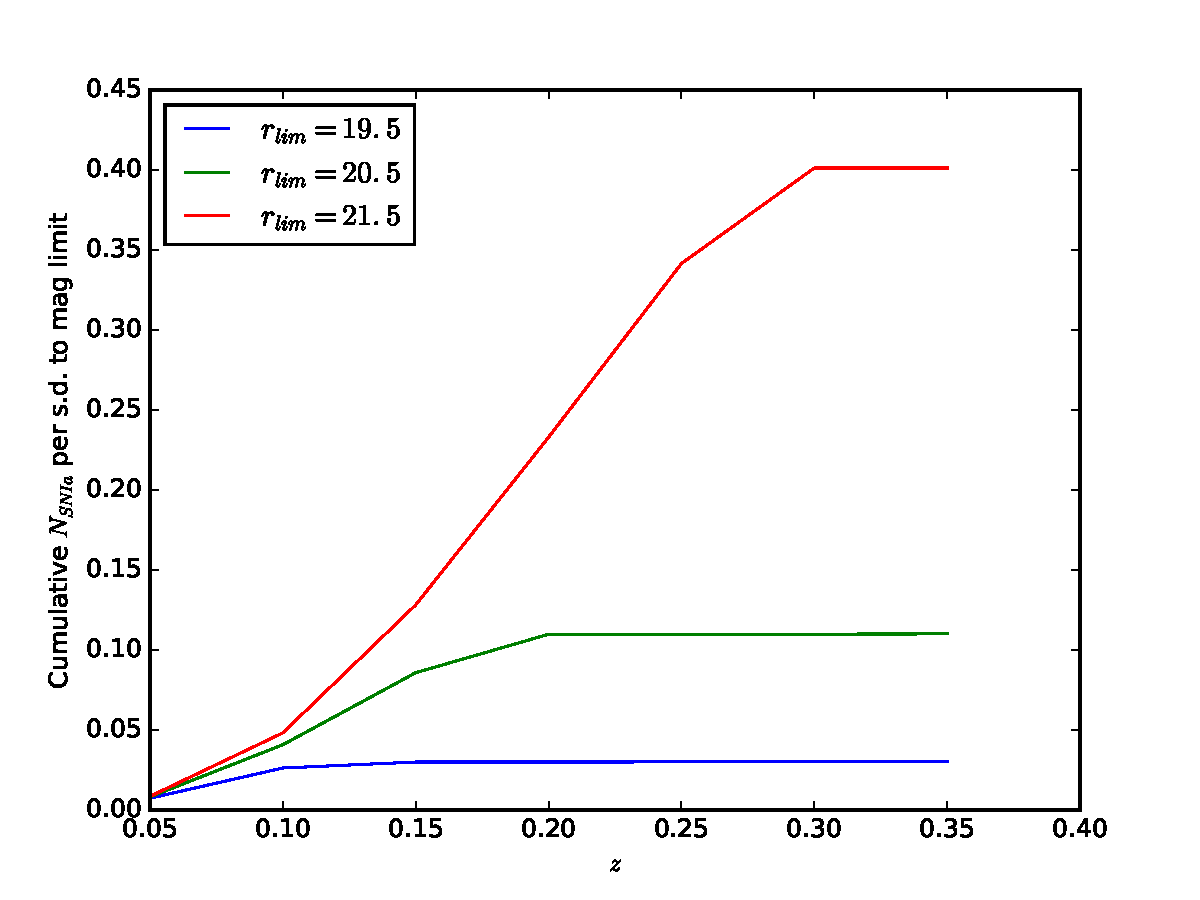
\includegraphics[width=8cm]{../src/cumulative.pdf}
\centering
\caption{Cumulative number densities as a function of redshift of SNe~Ia instantaneously brighter than several $r$ limiting magnitudes.
\label{cum:fig}}
\end{figure}

A ``passive'' way to trigger DESI observations of active supernovae is to request a fiber for the infrequent transient
that happens to occur in the field DESI is pointing at.  For an imaging survey that is complete to the DESI 
$z\sim0.3$ limit, the possible transient yield is then the number of DESI pointings multiplied by the number of objects per pointing.  For 10,000 pointings of the
main survey this is 2550 SNe~Ia.  Of these 750 would be below $z<0.15$ the discovery completeness limit of ZTF.  
For 6000 pointings of BGS the number is  90 SNe~Ia.  (The pointings are assumed to be taken with gaps longer than the longest SN~Ia control time.)
Most supernovae in the field, at higher redshifts, would not get a redshift.  The smaller number of supernovae at low-redshift, who have high apparent brightness
for a long time, would get a redshift.

An ``active'' way to trigger DESI observations of active supernovae
is to allocate a telescope pointing and fiber to an active transient.
The DESI surveys get filled in stochastically following
the random sky positions of transients.    If a transient occurs in a field that
has already achieved its full DESI depth, it is not targeted.
To get an idea of how many pointings could potentially be actively triggered, we examine the cumulative rate of observer-frame SN~Ia explosions as a function of redshift in Figure~\ref{total:fig}.  To $z= 0.3$, the SN~Ia classification limit of DESI, there are $0.3$ SNe~Ia per square degree per year or $2.25$ per footprint per year.
To $z= 0.2$, the SN~Ia discovery limit of ZTF, there are $0.08$ SNe~Ia per square degree per year or $0.6$ per footprint per year.  A large fraction of these
SNe beween $0.15<z<0.2$ will not be discovered by ZTF.
To $z=0.1$, the limit of good light-curves from ZTF, there are $0.02$ SNe~Ia per square degree per year or $0.15$ per footprint per year.  
Most fields of most imaging surveys cannot be monitored for
a full year so these numbers serve as an upper bound on the number of discovered supernovae with good light curves. 
The implication is that over the course of a year season, less than a quarter of DESI pointings will have ZTF SN~Ia transients.
The majority of fields do not have a transient. Can't predict which will.

\begin{figure}[h]
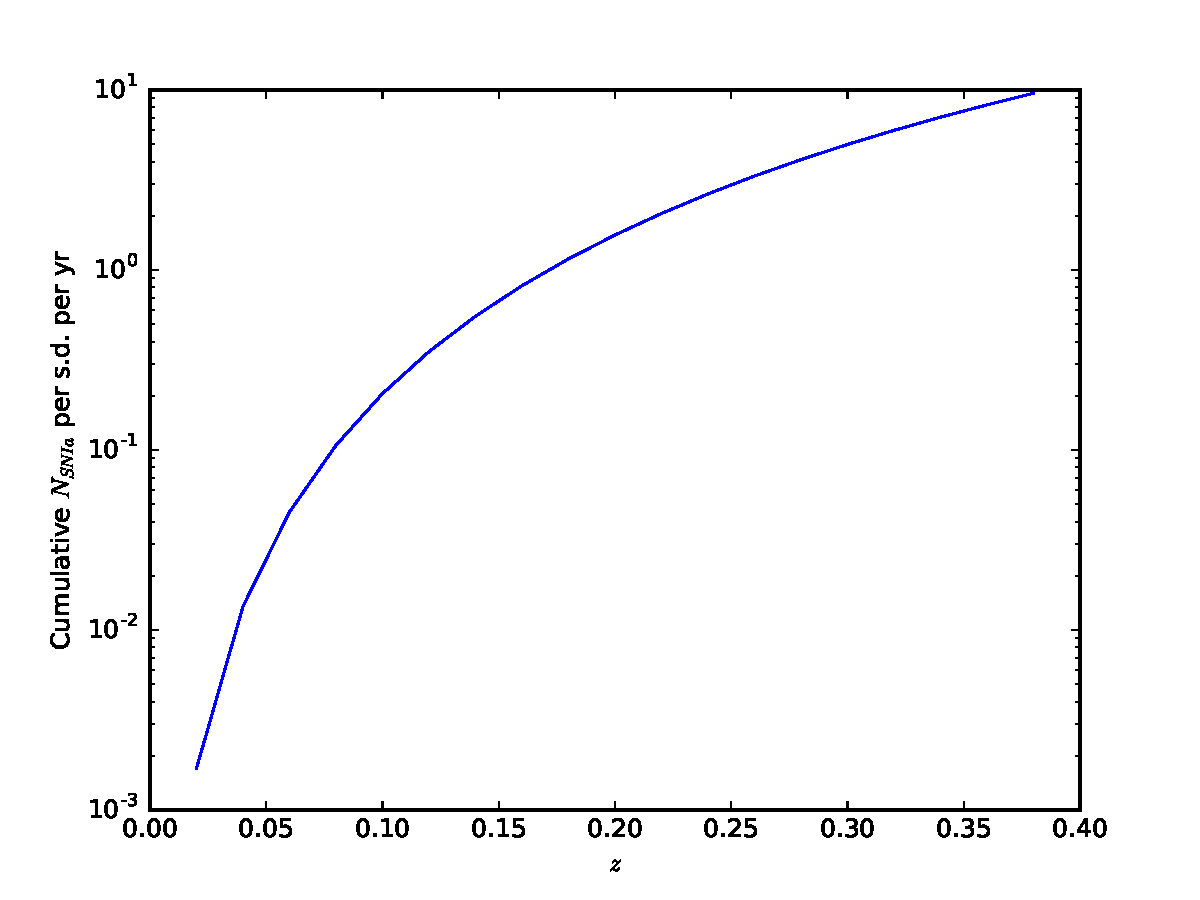
\includegraphics[width=8cm]{../src/total.pdf}
\centering
\caption{Cumulative rate of observer-frame SN~Ia explosions as a function of redshift. \label{total:fig}}
\end{figure}



Suppose the passive observing strategy were attached with a ZTF search. Ideally ZTF can arrange to have good light curves
for objects with DESI spectroscopic
classification.  ZTF anticipates 960/5 SNe~Ia per year with good light curves.
If coordination with ZTF is possible, there would remain $\sim 200/5$ supernovae with good light curves without DESI classification. 
Let us guesstimate $\sim 600/5$ without.  

If coordination with
ZTF is not possible, there will be some with a classification by virtue of happening to be active during a DESI pointing and allocated a fiber.




\section{Serendipitous Discovery of Active Type Ia Supernovae}
DESI can discover active SNe~Ia in the spectrum of a primary DESI target.
For now wait for properties of DESI galaxy targets and estimate rates based on those.  Figure~{cum:fig}, which shows the total number of 
supernovae in the field, shows an upper limit to the numbers of supernovae in DESI fibers.

\end{document} 
